\documentclass[tikz]{standalone}

\usepackage{tikz}
\usepackage{xcolor}
\usepackage{pgfplots}
\usepackage{../tikzviolinplots}
%\usepgfplotslibrary{external}
%\tikzexternalize
\usepackage{siunitx}
\usepackage{fontspec}
\pgfplotsset{compat=1.18}
\setmainfont{Source Serif 4}[
    Renderer = OpenType,
    SizeFeatures    = {%
        {Size={-9},Font=* Caption},
        {Size={9-13},Font=*},
        {Size={14-24},Font=* Subhead},
        {Size={24-},Font=* Display}
    },
    ItalicFeatures = {%
    SizeFeatures    = {%
            {Size={-9},Font=* Caption Italic},
            {Size={9-13},Font=* Italic},
            {Size={14-24},Font=* Subhead Italic},
            {Size={24-},Font=* Display Italic}
    },
    },
    BoldFeatures = {%
    SizeFeatures    = {%
            {Size={-9},Font=* Caption Semibold},
            {Size={9-13},Font=* Semibold},
            {Size={14-24},Font=* Subhead Semibold},
            {Size={24-},Font=* Display Semibold}
    },
    },
    BoldItalicFeatures = {%
    SizeFeatures    = {%
            {Size={-9},Font=* Caption Semibold Italic},
            {Size={9-13},Font=* Semibold Italic},
            {Size={14-24},Font=* Subhead Semibold Italic},
            {Size={24-},Font=* Display Semibold Italic}
    },
    },
    Numbers         = OldStyle,
]

\usetikzlibrary{shapes,arrows,positioning,backgrounds,calc,intersections,calc,svg.path,fit,fpu}
\definecolor{ugent-re}{RGB}{220, 78, 40}        % vermilion			/ vermiljoen
\definecolor{ugent-we}{RGB}{45, 140, 168}       % no match

\begin{document}
\begin{filecontents}[overwrite]{violin-small.dat}
    A,B,C,D,E
    0.001,0.001,0.001,0.001,0.001
    0.0006,0.0009,0.001,0.0009,0.0014
    -0.0109,-0.0068,-0.0036,-0.0034,-0.0012
    0.001,0.0103,0.0162,0.0167,0.0209
    0.001,0.0129,0.0156,0.0164,0.0204
    0.001,0.001,0.001,0.001,0.001
    0.001,0.001,0.001,0.001,0.001
    0.001,0.001,0.001,0.001,0.001
    0.001,0.001,0.001,0.001,0.001
    0.001,0.001,0.001,0.001,0.001
    0.001,0.001,0.001,0.001,0.001
    0.001,0.001,0.001,0.001,0.001
    0.001,0.001,0.001,0.001,0.001
    -0.0099,-0.0052,-0.0019,-0.0017,-0.0002
    0.001,0.001,0.001,0.001,0.001
    0.001,0.001,0.001,0.001,0.001
    0.001,0.001,0.001,0.001,0.001
    0.001,0.001,0.001,0.001,0.001
    0.001,0.001,0.001,0.001,0.001
    0.0029,0.0022,0.0017,0.0008,0.0011
    0.001,0.001,0.001,0.001,0.001
    0.001,0.0009,0.001,0.001,0.001
    0.0013,0.0012,0.0014,0.0014,0.0015
    0.001,0.001,0.001,0.001,0.001
    0.001,0.001,0.001,0.001,0.001
    0.001,0.001,0.001,0.001,0.001
    0.001,0.001,0.001,0.001,0.001
    -39.709,-58.3352,-59.6559,-62.8441,-79.6688
    0.001,0.001,0.001,0.001,0.001
    0.001,0.001,0.001,0.001,0.001
    0.001,0.001,0.001,0.001,0.001
    0.0011,0.001,0.001,0.001,0.001
    0.001,0.001,0.001,0.001,0.001
    0.001,0.001,0.0009,0.0009,0.0009
    -0.0176,-0.0109,-0.0068,-0.0055,-0.002
    -0.0534,-0.0261,-0.0036,0.003,0.0181
    0.001,0.001,0.001,0.001,0.001
    0.0017,0.0012,0.0012,0.0016,0.0016
    0.001,0.001,0.001,0.001,0.001
    -0.1281,-0.0845,-0.0691,-0.0534,-0.0483
    0.001,0.001,0.001,0.001,0.001
    0.002,0.0014,0.0018,0.0026,0.0034
    0.001,0.001,0.001,0.001,0.001
    0.0008,0.0056,0.0091,0.0099,0.0143
    0.001,0.001,0.001,0.001,0.001
    -0.0034,-0.0046,-0.0036,-0.0033,-0.0018
    -0.0149,0.1804,0.2623,0.3229,0.4342
    0.001,0.001,0.001,0.001,0.001
    0.001,0.001,0.001,0.001,0.001
    0.001,0.001,0.001,0.001,0.001
    -0.0283,-0.0226,-0.0171,-0.0156,-0.0112
    0.001,0.001,0.001,0.001,0.001
    0.001,0.001,0.001,0.001,0.001
    0.001,0.001,0.001,0.001,0.001
    0.001,0.001,0.001,0.001,0.001
    -34.076,-61.3935,-62.7912,-65.7993,-84.1827
    0.001,0.001,0.001,0.001,0.001
    0.001,0.001,0.001,0.001,0.001
    0.0003,0.0038,0.0062,0.0078,0.012
    -0.0152,-0.0155,-0.0151,-0.0158,-0.0125
    -0.0172,-0.0108,-0.0088,-0.0058,-0.0013
    21.2637,-30.8697,-33.9761,-43.1811,-56.2711
    0.001,0.001,0.001,0.001,0.001
    0.0012,0.0011,0.0012,0.0012,0.0014
    0.0,-0.007,-0.0031,-0.0047,-0.0011
    0.001,0.001,0.001,0.001,0.001
    0.0005,0.0005,0.0009,0.001,0.0012
    -18.2378,-18.9811,-16.8418,-16.7692,-15.8083
    0.001,0.001,0.001,0.001,0.001
    0.001,0.001,0.001,0.001,0.001
    -0.0015,0.0011,0.0037,0.0056,0.0102
    0.0012,0.0009,0.0009,0.001,0.0013
    0.001,0.001,0.001,0.001,0.001
    0.001,0.0054,0.0077,0.0089,0.013
    0.001,0.001,0.001,0.001,0.001
\end{filecontents}
\begin{tikzpicture}
    \pgfplotsset{height=5cm,width=6cm}
    \pgfkeys{/pgfplots/yticklabel={\addfontfeature{Numbers={Lining}}\qty[round-mode=places, round-precision=0]{\tick}{\mega{}}},}
    \violinsetoptions[
        scaled,
        averages,
    ]{
        xmin=0.3,xmax=6.2,
        ymin=-110,ymax=40,
        xlabel style={
            yshift = {-3*height("a")}
        },
        ymajorgrids=true,
        ytick distance=30,
        ylabel={№ of blocks}
    }
    \violinplot[%
        index=A,
        relative position=1,
        label={30},
        samples=100,
        average mark=*,
        average fill=black,
        average fill opacity=1.0,
        average size=1pt,
        color=ugent-we,
    ]{violin-small.dat}
    \violinplot[%
        index=B,
        relative position=2.2,
        label={60},
        samples=100,
        average mark=*,
        average fill=black,
        average fill opacity=1.0,
        average size=1pt,
        color=ugent-we,
    ]{violin-small.dat}
    \violinplot[%
        index=C,
        relative position=3.3,
        label={90},
        samples=100,
        average mark=*,
        average fill=black,
        average fill opacity=1.0,
        average size=1pt,
        color=ugent-we,
    ]{violin-small.dat}
    \violinplot[%
        index=D,
        relative position=4.4,
        label={120},
        samples=100,
        average mark=*,
        average fill=black,
        average fill opacity=1.0,
        average size=1pt,
        color=ugent-we,
    ]{violin-small.dat}
    %! parser = off
    \pgfkeys{
        /pgfplots/xticklabels={\addfontfeature{Numbers={OldStyle,Proportional}}\textsc{asap}},
        /pgfplots/xlabel={Execution models (\textsc{em-})},
    };
    %! parser = on
    \violinplot[%
        index=E,
        relative position=5.5,
        samples=100,
        average mark=*,
        average fill=black,
        average fill opacity=1.0,
        average size=1pt,
    ]{violin-small.dat}
\end{tikzpicture}
\end{document}
